\documentclass[12pt, a4paper]{article}

\usepackage[utf8]{inputenc}
\usepackage[russian]{babel}
\usepackage{geometry}
\usepackage{mathtools}
\usepackage{verbatim}
\usepackage{indentfirst}
\usepackage{caption}
\usepackage{subcaption}
\usepackage{import}
\usepackage{xifthen}
\usepackage{pdfpages}
\usepackage{transparent}
\usepackage{graphicx}
\usepackage{caption}
\usepackage{hyperref}
\usepackage{float}

\newcommand{\norm}[1]{\lVert #1 \rVert}
\newcommand{\abs}[1]{\lvert #1 \rvert}
\usepackage[oglav,spisok,boldsect,eqwhole,figwhole,hyperref,hyperprint,remarks,greekit]{./style/fn2kursstyle}

\graphicspath{{./style/}{./figures/}}

\frenchspacing

\title{Решение задач интерполирования}
\lab{4}
\author{М.\,А.~Каган}
\creator{И.\,А.~Яковлев}
\supervisor{}
\group{ФН2-51Б}
\date{2024}

\begin{document}
	\maketitle
	\tableofcontents
	
	\newpage
	

	
	\section-{Контрольные вопросы}
	
	\begin{enumerate}
	\item \textbf{Определите количество арифметических операций, требуемое для интерполирования функции в некоторой точке многочленом Лагранжа (включая построение самого многочлена) на сетке с числом узлов, равным n.}
	
	\vspace*{0.2cm}
	
	\textit{\textbf{Ответ:}}
	
	Для построения интерполяционного многочлена в форме Ньютона, необходимо посчитать следующую таблицу разделенных разностей:
	\begin{figure}[ht]
		\centering
		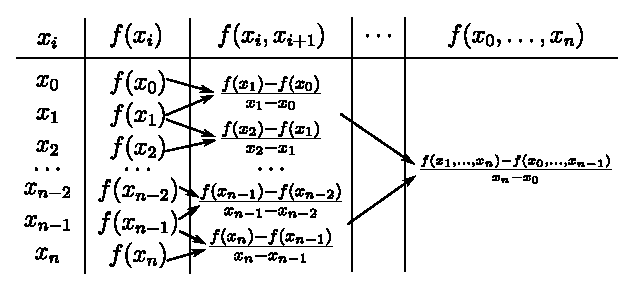
\includegraphics[scale=1.35]{таблица1.eps}
	\end{figure}
	
	В каждом последующем столбце количество строк уменьшается на одну, поскольку, чтобы посчитать значение  $f(x_i, \ldots, x_{i+k})$ с учетом того, что все необходимые коэффициенты известны, необходимо совершить одну операцию деления. Таким образом, нужно произвести $\sfrac{n(n-1)}{2} - n$ операций.
	
	Многочлен в форме Ньютона можно записать в виде:
	\[
	L_n(x) = f(x_0) + (x - x_0)f(x_1) + \ldots + (x - x_0)\ldots (x - x_n)f(x_n). 
	\]
	Точка $\tilde{x}$ --- точка, в которой необходимо вычислить значение функции $L_n(x)$. Так как все разделенные разности известны, остается вычислить множители:
	 \[
	 f(x_0,x_1, \ldots,x_{k+1})\prod\limits_{j = 0}^{k}(\tilde{x} - x_j)
	 \]
	где $k = 0, \ldots, n-1$. Если сохранять промежуточные вычисления $\prod\limits_{j = 0}^{k}(\tilde{x} - x_j)$, то количество операций умножения равняется $n$. 
	
	Таким образом общее количество необходимых операций: $\sfrac{n(n-1)}{2}$
	
	\item \textbf{Определите количество арифметических операций, требуемое для интерполирования функции в некоторой точке кубическим сплайном (включая затраты на вычисление коэффициентов сплайна) на сетке с числом узлов, равным n.}
	\vspace*{0.2cm}
	
	\textit{\textbf{Ответ:}}
	
	
		
	\item \textbf{Функция $f(x) = e ^ x$ интерполируется многочленом Лагранжа на отрезке $[0, 2]$ на равномерной сетке с шагом $h=0.2$.Оцените ошибку экстраполяции в точке $x = 2.2$, построив многочлен Лагранжа и подставив в него это значение, а также по формуле для погрешности экстраполяции.}
	\vspace*{0.2cm}

	\textit{\textbf{Ответ:}}
	
	Погрешность с помощью прямых вычислений: $1.59 \cdot 10^{-7}$.
	
	Погрешность с помощью формулы:
	\[
	\abs{f(2.2) - L_n(2.2)} \le \dfrac{M_{n+1}}{(n+1)!}\abs{\omega(2.2)} \approx 1.85 \cdot 10^{-7},
	\]
	где $M_{n+1} = \norm{f^{(n+1)}(x)}_C$ и $\omega(x) = \prod\limits_{k=0}^{n}(x - x_k)$
	
	\item \textbf{}
	\vspace*{0.2cm}
	
	\textit{\textbf{Ответ:}}
	
	\item \textbf{Каковы достоинства и недостатки сплайн-интерполяции и интерполяции многочленом Лагранжа?}
	\vspace*{0.2cm}
	
	\textit{\textbf{Ответ:}}
	
	\item \textbf{}
	\vspace*{0.2cm}
	
	\textit{\textbf{Ответ:}}
	\end{enumerate}
	



	
\end{document}